\documentclass[a4paper,12pt]{article}
\usepackage[T2A]{fontenc}
\usepackage[utf8]{inputenc}
\usepackage[english,russian]{babel}
\usepackage{listings}

\usepackage{amsmath}
\usepackage{MnSymbol}
\usepackage{wasysym}
\usepackage{indentfirst}
\usepackage[unicode, pdftex]{hyperref}

\usepackage{pgfplots}
\pgfplotsset{compat=1.9}

\usepackage{geometry}
\geometry{left=2cm}
\geometry{right=1.5cm}
\geometry{top=1cm}
\geometry{bottom=2cm}

\usepackage{graphicx}
\graphicspath{{img/}}
\DeclareGraphicsExtensions{.pdf,.png,.jpg}

\newcommand{\anonsection}[1]{\section*{#1}\addcontentsline{toc}{section}{#1}}

% переименовываем  список литературы в "список используемой литературы"
\addto\captionsrussian{\def\refname{Список используемой литературы}}

\usepackage{float}

\lstset{
    language=C++,
    numbers=left,
    frame=single,
    texcl=true,
    basicstyle=\ttfamily
}

\begin{document}

\begin{titlepage}

    \begin{center}
        \large
        Государственное образовательное учреждение высшего профессионального образования\\
        “Московский государственный технический университет имени Н.Э.Баумана”
        \vspace{3cm}

        \textsc{Дисциплина: Анализ алгоритмов}
        \vspace{0.5cm}

        \textsc{Лабораторная работа №3}
        \vspace{3cm}

        {\LARGE ТРУДОЕМКОСТЬ СОРТИРОВОК}
        \vspace{3cm}

        Студент группы ИУ7-53,\\
        Степанов Александр Олегович
        \vfill
    \end{center}

    \begin{flushright}
        \begin{tabular}{l}
            Преподаватели:\\
            Строганов Юрий Владимирович\\
            Волкова Лилия Леонидовна
        \end{tabular}
    \end{flushright}

    \begin{center}

        2019 г.

    \end{center}

\end{titlepage}

\tableofcontents

\newpage
\anonsection{Введение}

В настоящее время необходимо сортировать большие объемы данных. Для этой
цели существуют алгоритмы сортировки, которые упорядочивают элементы в
списке \cite{knuth}. Алгоритмы сортировки могут использоваться для ускорения поиска элементов
среди большого количества информации, например для баз данных или математических программ.
Также сортировки могут быть полезны в сферах бизнеса и бухгалтерии.

Целями данной лабораторной работы является:

\begin{enumerate}
    \item реализовать три различных алгоритма сортировки;
    \item теоретически вычислить эффективность алгоритмов;
    \item сравнить алгоритмы по времени и памяти.
\end{enumerate}

\newpage
\section{Аналитическая часть}

Алгоритмы сортировки имеют большое практическое применение. Их можно встретить почти везде,
где речь идет об обработке и хранении больших объемов информации. Некоторые задачи обработки
данных решаются проще, если данные упорядочены.

\subsection{Описание задачи}

\textbf{Сортировка} - это процесс упорядочения некоторого множества элементов,
на котором определены отношения порядка >, <, >=, <= (по возрастанию или убыванию) \cite{pav}.
При выборе алгоритма сортировки необходимо выбрать тот алгоритм, который будет проделывать
минимум операций над данными и тем самым максимально быстро получать необходимый результат -
отсортированный список.

\textbf{Трудоемкость алгоритма} - это зависимость количества операций от количества
данных, с которыми алгоритм работает. Список действий, цена которых считается за 1:

$$
+, -, *, /, \%, =, ==, !=, <, >, <=, >=, [], +=
$$

На данный момент существует большое количесво алгоритмов сортировки, которые отличаются
своей трудоемкостью \cite{knuth}. Первые прототипы современных методов сортировки появились уже
в XIX веке. К 1890 году для ускорения обработки данных переписи населения в США американец
Герман Холлерит создал первый статистический табулятор — электромеханическую машину,
предназначенную для автоматической обработки информации, записанной на перфокартах
\cite{eniac}.
В дальнейшем история алгоритмов оказалась связана с развитием электронно-вычислительных машин.

За последние 70 лет появилось множество алгоритмов сортировок для компьютера.\cite{knuth}

\subsection{Выводы}

В данной работе стоит задача реализации 3 алгоритмов сортировки: сортировка пузырьком,
шейкером и быстрая сортировка. Необходимо теоретически оценить трудоемкость этих алгоритмов
и проверить все вычисления экспериментально.

\newpage
\section{Конструкторская часть}

Рассмотрим сортировку пузырьком, шейкером и быструю сортировку.

\subsection{Функциональная модель}

На рисунке \ref{img:IDEF0} представлена функциональная модель IDEF0 уровня 1.

\begin{figure}[H]
    \centering
    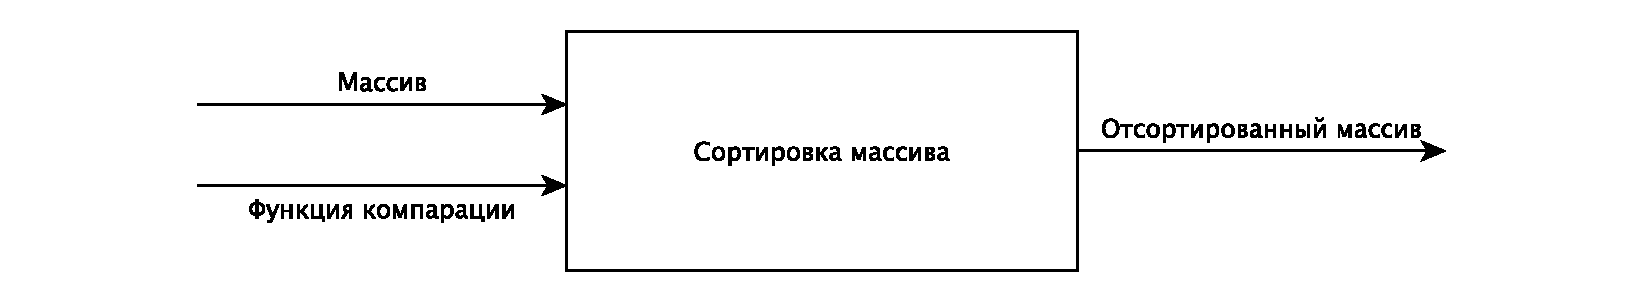
\includegraphics[scale=0.5]{IDEF0}
    \caption{Функциональная модель IDEF0 уровня 1}
    \label{img:IDEF0}
\end{figure}

\subsection{Схемы алгоритмов}

На рисунке \ref{img:bubble} изображена схема алгоритма сортировки пузырьком.

\begin{figure}[H]
    \centering
    \includegraphics[scale=0.55]{Bubble}
    \caption{Сортировка пузырьком}
    \label{img:bubble}
\end{figure}

На рисунке \ref{img:shaker} изображена схема алгоритма сортировки шейкером.

\begin{figure}[H]
    \centering
    \includegraphics[scale=0.8]{Shaker}
    \caption{Сортировка шейкером}
    \label{img:shaker}
\end{figure}

На рисунке \ref{img:qsort} изображена схема алгоритма быстрой сортировки.

\begin{figure}[H]
    \centering
    \includegraphics[scale=0.45]{QSort}
    \caption{Быстрая сортировка}
    \label{img:qsort}
\end{figure}

Произведем теоретическую оценку трудоемкости алгоритмов сортировки

\begin{enumerate}
    \item \textbf{Сортировка пузырьком}

        В лучшем случае, когда массив будет отсортирован, трудоемкость будет считать
        по формуле \ref{eq:bubble-good}.

        \begin{equation}\label{eq:bubble-good}
            f = 1 + 2N + \frac{N(N-1)}{2} \cdot 6 =
            3N^2 - N + 1
        \end{equation}

        В худшем случае, когда массив будет обратно отсортирован, трудоемкость будет
        считаться по формуле \ref{eq:bubble-bad}.

        \begin{equation}\label{eq:bubble-bad}
            f = 1 + 2N + \frac{N(N-1)}{2} \cdot 11 =
            \frac{11}{2}N^2 - \frac{7}{2}N + 1
        \end{equation}

        И в лучшем, и в худшем случае, сортировка пузьком имеет трудоемкость $O(N^2)$.

    \item \textbf{Сортировка шейкером} \cite{knuth}

        И в лучшем, и в худшем случае, сортировка шейкером иммет трудоемкость $O(N^2)$

    \item \textbf{Быстрая сортировка} \cite{knuth}

        В лучшем случае, когда массив упорядочен, трудоемкость равна $O(N \cdot \ln(N))$.

        В худшем случае, когда массив обратно упорядочен, трудоемкость равна $O(N^2)$.
\end{enumerate}

\subsection{Выводы}

Сортировка пузырьком и сортировка шейкером имеют одинаковую трудоемкость $O(N^2)$, но
по коэффициентам видно, что шейкерная сортировка быстрее пузырька в 4 раза. Быстрая
сортировка имеет трудоемкость $O(N \cdot \ln(N))$ из чего можно сделать вывод, что
быстрая сортировка на порядок быстрее двух других.

\newpage
\section{Технологическая часть}

Необходимо выбрать средства для разработки алгоритмов и подготовить тесты.

\subsection{Требования к программному обеспечению}

Программное обеспечение должно обеспечивать замер процессорного времени выполнения каждого
алгоритма. Проводятся замеры для случайно генерируемых массивов размерности до 10000.

\subsection{Средства реализации}

В качестве языка программирования был выбран C++. Данный язык имеет высокую скорость и
богатую стандартную библиотеку, содержащую необходимые контейнеры для данной работы.
Программа, написанная на C++, будет доступна на всех платформах.

Время замерялось с помощью библиотеки chrono, которая измеряет процессорное
время \cite{chrono}.

\subsection{Листинг кода}

Результаты разработки указаны на листингах \ref{list:bubble}, \ref{list:shaker},
\ref{list:qsort}.

\begin{lstlisting}[caption=Сортировка пузырьком,label=list:bubble]
template < typename Type >
void BubbleSort< Type >::sort(std::vector< Type >& array,
                              bool (*comp)(Type, Type))
{
    for (int i = 0; i < array.size(); ++i) {
        for (int j = 0; j < array.size() - i - 1; ++j) {
            if (comp(array[j], array[j + 1])) {
                std::swap(array[j], array[j + 1]);
            }
        }
    }
}
\end{lstlisting}

\begin{lstlisting}[caption=Сортировка шейкером,label=list:shaker]
template < typename Type >
void ShakerSort< Type >::sort(std::vector< Type >& array,
                              bool (*comp)(Type, Type))
{
    int left = 0;
    int right = array.size() - 1;

    while (left <= right) {
        for (int i = left; i < right; ++i) {
            if (comp(array[i], array[i + 1])) {
                std::swap(array[i], array[i + 1]);
            }
        }
        --right;

        for (int i = right; i > left; --i) {
            if (comp(array[i - 1], array[i])) {
                std::swap(array[i - 1], array[i]);
            }
        }
        ++left;
    }
}
\end{lstlisting}

\begin{lstlisting}[caption=Быстрая сортировка,label=list:qsort]
template < typename Type >
void QSort< Type >::recursive(std::vector< Type >& array,
                              int start, int finish,
                              bool (*comp)(Type, Type))
{
    if (start < finish) {
        int left = start, right = finish;
        Type middle = array[(left + right) >> 1];

         while (left <= right) {
            while (comp(middle, array[left])) left++;
            while (comp(array[right], middle)) right--;

            if (left <= right) {
                std::swap(array[left], array[right]);
                ++left;
                --right;
            }
        }

        if (start < right) recursive(array, start, right, comp);
        if (left < finish) recursive(array, left, finish, comp);
    }
}
\end{lstlisting}

\subsection{Тестирование}

Для тестирования программы были заготовлены следующие тесты на таблице \ref{table:test}.

\begin{table}[H]
    \centering
    \caption{Тесты для алгоритмов}
    \label{table:test}
    \begin{tabular}{|c|c|}
        \hline
        Входной массив & Ожидаемый результат \\
        \hline
        1, 2, 3, 4, 5, 6, 7, 8, 9 & 1, 2, 3, 4, 5, 6, 7, 8, 9 \\
        \hline
        9, 8, 7, 6, 5, 4, 3, 2, 1 & 1, 2, 3, 4, 5, 6, 7, 8, 9 \\
        \hline
        4, 2, 7, 4, 8, 2, 4, 8, 1 & 1, 2, 2, 4, 4, 4, 7, 8, 8 \\
        \hline
        5, 5, 5, 5, 5, 5, 5, 5, 5 & 5, 5, 5, 5, 5, 5, 5, 5, 5 \\
        \hline
    \end{tabular}
\end{table}

\subsection{Выводы}

Для сравнения были реализованы 3 алгоритма на выбранном языке
программирования C++. Чтобы проверить правильность работы алгоритмов
были подготовлены тесты.

\newpage
\section{Экспериментальная часть}

Проведем тестирование и сравним алгоритмы по времени работы.

\subsection{Примеры работ}

Ниже приведены примеры работ при корректных и некорректных данных.

\begin{figure}[H]
    \centering
    
\includegraphics[scale=0.4]{zero_arg}
    \caption{Без аргументов}
    \label{img:zero-arg}
\end{figure}

\begin{figure}[H]
    \centering
    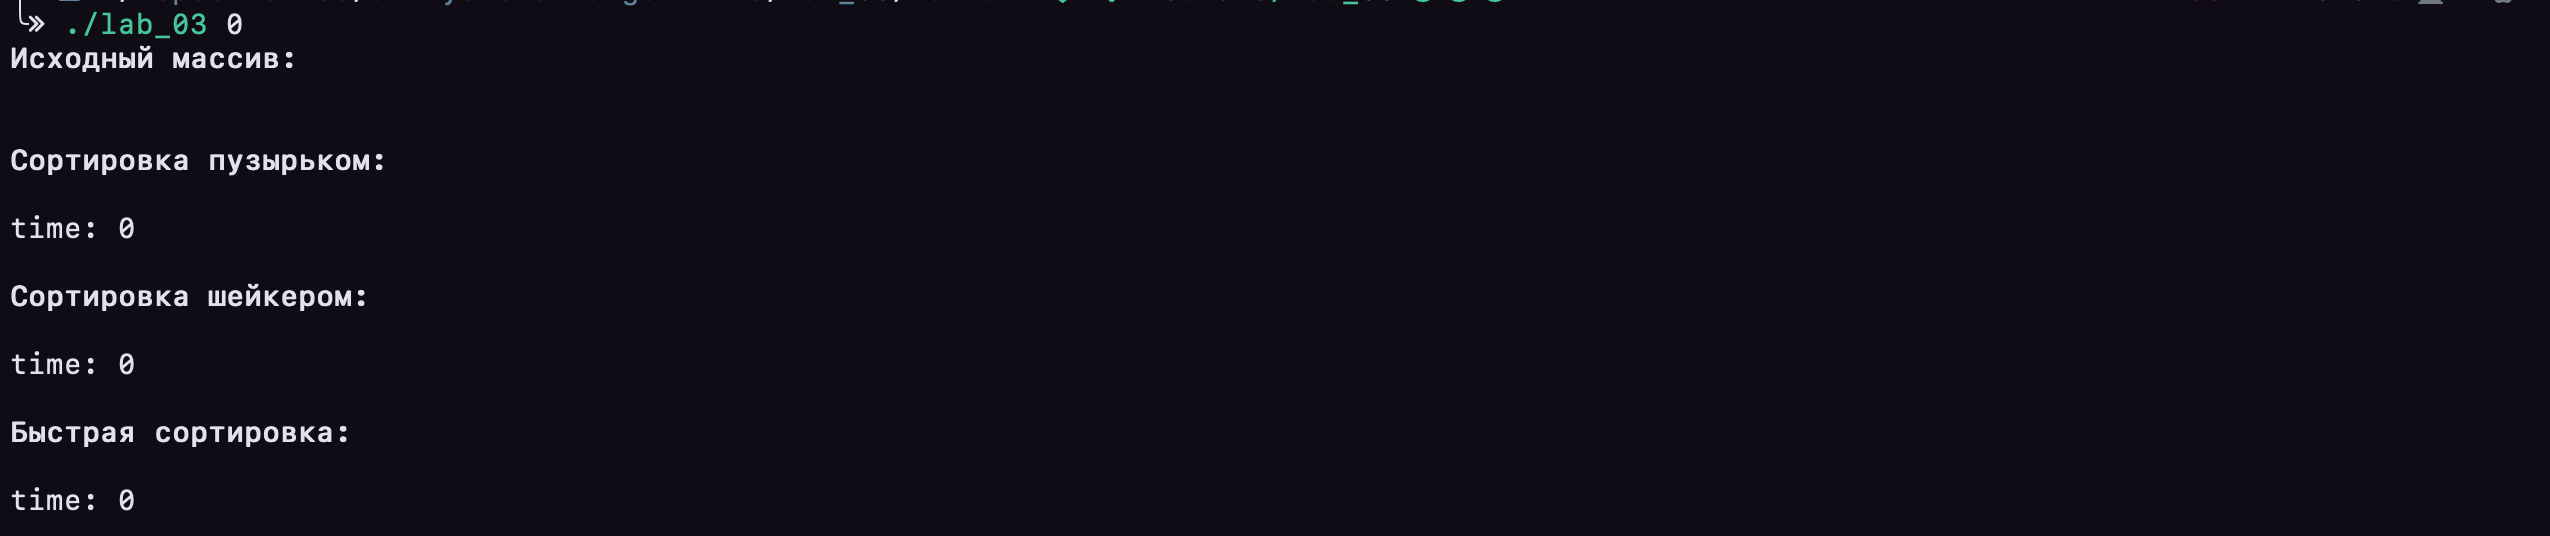
\includegraphics[scale=0.4]{zero}
    \caption{Ноль в аргументе}
    \label{img:zero}
\end{figure}

\begin{figure}[H]
    \centering
    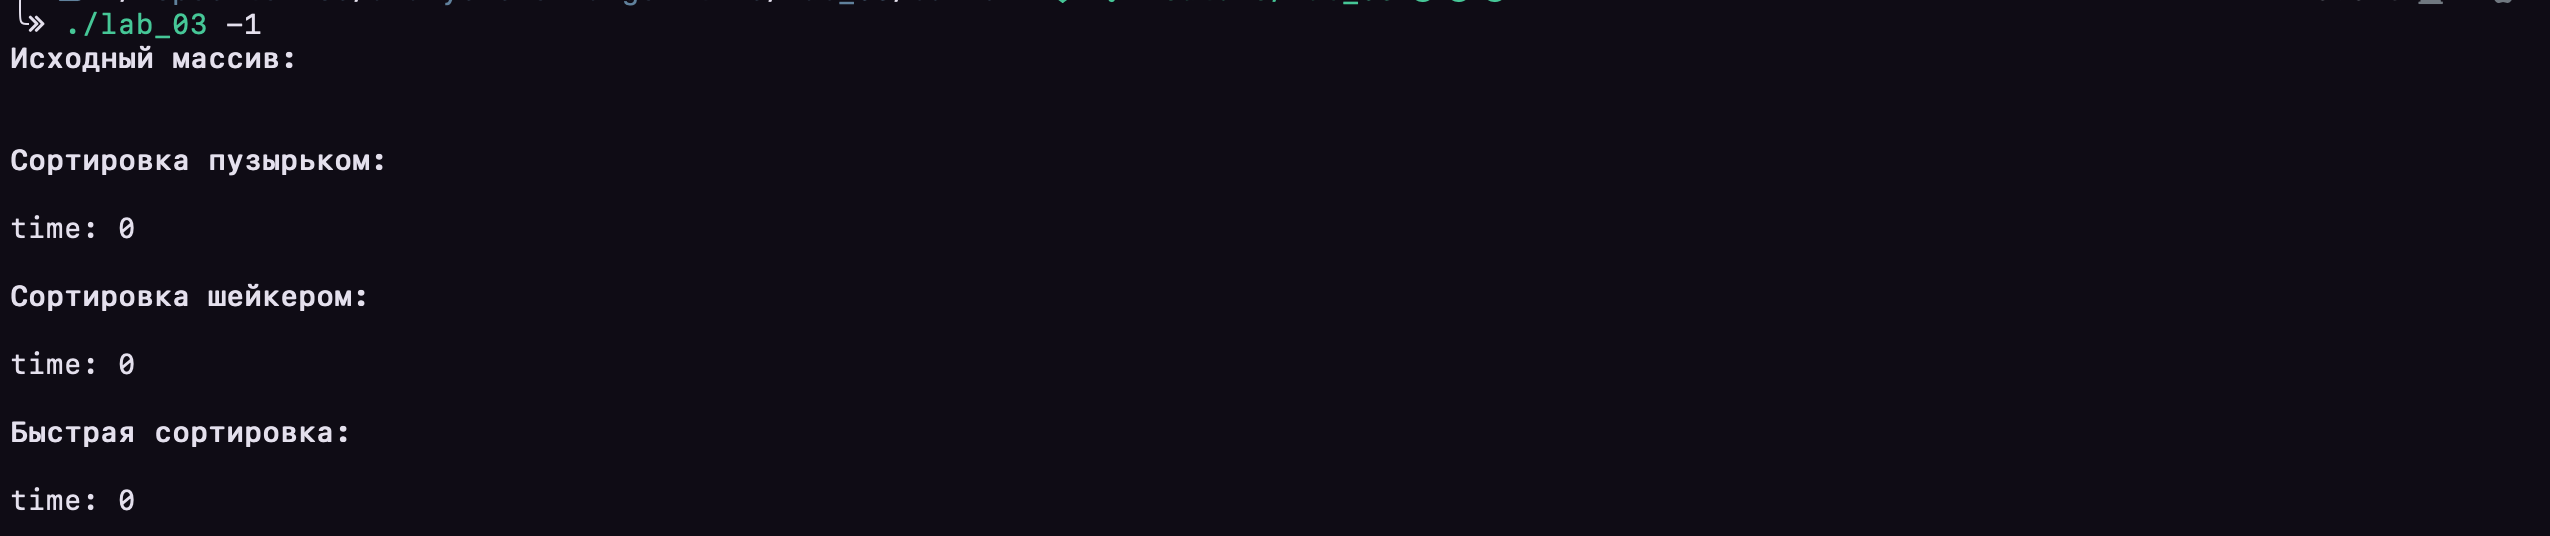
\includegraphics[scale=0.4]{less_zero}
    \caption{Меньше нуля в аргументе}
    \label{img:less-zero}
\end{figure}

\begin{figure}[H]
    \centering
    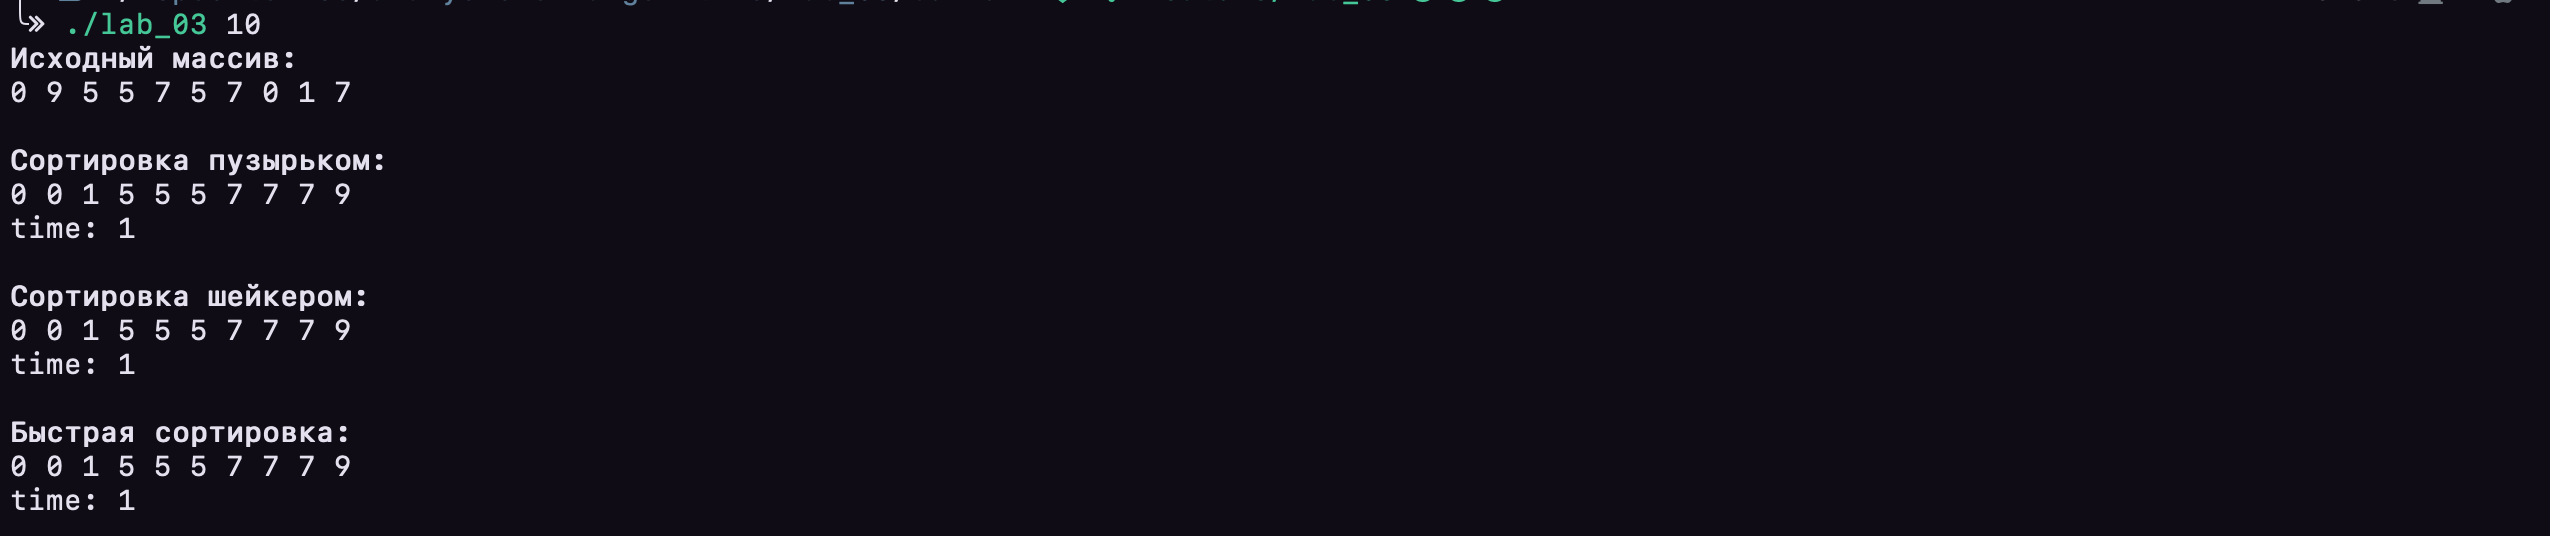
\includegraphics[scale=0.4]{normal}
    \caption{Корректный аргумент}
    \label{img:normal}
\end{figure}

\subsection{Результаты тестирования}

Для тестирования были использованы тесты из таблицы \ref{table:test}.
Результаты продемонстрированы на таблицах \ref{table:bubble}, \ref{table:shaker},
\ref{table:qsort}.

\begin{table}[H]
    \centering
    \caption{Результаты тестирования сортировки пузырьком}
    \label{table:bubble}
    \begin{tabular}{|c|c|}
        \hline
        Входной массив & Результат \\
        \hline
        1, 2, 3, 4, 5, 6, 7, 8, 9 & 1, 2, 3, 4, 5, 6, 7, 8, 9 \\
        \hline
        9, 8, 7, 6, 5, 4, 3, 2, 1 & 1, 2, 3, 4, 5, 6, 7, 8, 9 \\
        \hline
        4, 2, 7, 4, 8, 2, 4, 8, 1 & 1, 2, 2, 4, 4, 4, 7, 8, 8 \\
        \hline
        5, 5, 5, 5, 5, 5, 5, 5, 5 & 5, 5, 5, 5, 5, 5, 5, 5, 5 \\
        \hline
    \end{tabular}
\end{table}

\begin{table}[H]
    \centering
    \caption{Результаты тестирования сортировки шейкером}
    \label{table:shaker}
    \begin{tabular}{|c|c|}
        \hline
        Входной массив & Результат \\
        \hline
        1, 2, 3, 4, 5, 6, 7, 8, 9 & 1, 2, 3, 4, 5, 6, 7, 8, 9 \\
        \hline
        9, 8, 7, 6, 5, 4, 3, 2, 1 & 1, 2, 3, 4, 5, 6, 7, 8, 9 \\
        \hline
        4, 2, 7, 4, 8, 2, 4, 8, 1 & 1, 2, 2, 4, 4, 4, 7, 8, 8 \\
        \hline
        5, 5, 5, 5, 5, 5, 5, 5, 5 & 5, 5, 5, 5, 5, 5, 5, 5, 5 \\
        \hline
    \end{tabular}
\end{table}

\begin{table}[H]
    \centering
    \caption{Результаты тестирования быстрой сортировки}
    \label{table:qsort}
    \begin{tabular}{|c|c|}
        \hline
        Входной массив & Результат \\
        \hline
        1, 2, 3, 4, 5, 6, 7, 8, 9 & 1, 2, 3, 4, 5, 6, 7, 8, 9 \\
        \hline
        9, 8, 7, 6, 5, 4, 3, 2, 1 & 1, 2, 3, 4, 5, 6, 7, 8, 9 \\
        \hline
        4, 2, 7, 4, 8, 2, 4, 8, 1 & 1, 2, 2, 4, 4, 4, 7, 8, 8 \\
        \hline
        5, 5, 5, 5, 5, 5, 5, 5, 5 & 5, 5, 5, 5, 5, 5, 5, 5, 5 \\
        \hline
    \end{tabular}
\end{table}

Все тесты пройдены успешно.

\subsection{Замеры времени}

На рисунке \ref{img:front} представлены результаты замера времени для отсортированного
массива, на рисунке \ref{img:back} - для обратно отсортированного и на рисунке
\ref{img:random} - для случайно сгенерированного массива.

\begin{figure}[H]
    \begin{tikzpicture}
        \begin{axis}[
            legend pos = north west,
            xlabel=Размер массива,
            ylabel=микросекунды,
            grid = major,
            width = 0.8\paperwidth,
            height = 0.38\paperheight,
            line width = 1
        ]
            \legend{
                Сортировка пузырьком,
                Сортировка шейкером,
                Быстрая сортировка
            };
            \addplot[black] coordinates {
                (100, 54)
                (200, 480)
                (300, 990)
                (400, 1931)
                (500, 3256)
                (600, 5198)
                (700, 7921)
                (800, 11294)
                (900, 15785)
                (1000, 21199)
                (1100, 27480)
                (1200, 35323)
                (1300, 44344)
                (1400, 54314)
                (1500, 66169)
                (1600, 79273)
                (1700, 94383)
                (1800, 111104)
                (1900, 130147)
                (2000, 151057)
                (2100, 174071)
                (2200, 199279)
                (2300, 226997)
                (2400, 256903)
                (2500, 289446)
                (2600, 324843)
                (2700, 362309)
                (2800, 402484)
                (2900, 445472)
                (3000, 491389)
                (3100, 543209)
                (3200, 595428)
                (3300, 651489)
                (3400, 710303)
                (3500, 772716)
                (3600, 838642)
                (3700, 908582)
                (3800, 982140)
                (3900, 1061740)
                (4000, 1143214)
                (4100, 1228776)
                (4200, 1318504)
                (4300, 1412610)
                (4400, 1510895)
                (4500, 1616530)
                (4600, 1724451)
                (4700, 1836661)
                (4800, 1953636)
                (4900, 2075992)
                (5000, 2205651)
                (5100, 2338098)
                (5200, 2475531)
                (5300, 2620596)
                (5400, 2769172)
                (5500, 2922693)
                (5600, 3082142)
                (5700, 3249057)
                (5800, 3420220)
                (5900, 3597278)
                (6000, 3782922)
                (6100, 3972604)
                (6200, 4183597)
                (6300, 4413195)
                (6400, 4622532)
                (6500, 4845889)
                (6600, 5067437)
                (6700, 5295290)
                (6800, 5532806)
                (6900, 5774709)
                (7000, 6025377)
                (7100, 6281631)
                (7200, 6546718)
                (7300, 6817305)
                (7400, 7099640)
                (7500, 7385160)
                (7600, 7680146)
                (7700, 7981127)
                (7800, 8292025)
                (7900, 8610959)
                (8000, 8935735)
                (8100, 9270524)
                (8200, 9612418)
                (8300, 9966500)
                (8400, 10325515)
                (8500, 10693856)
                (8600, 11071532)
                (8700, 11455318)
                (8800, 11851570)
                (8900, 12255031)
                (9000, 12667819)
                (9100, 13088573)
                (9200, 13519645)
                (9300, 13960276)
                (9400, 14412407)
                (9500, 14873914)
                (9600, 15343144)
                (9700, 15822843)
                (9800, 16312289)
                (9900, 16811542)
                (10000, 17320621)
            };

            \addplot[dashed] coordinates {
                (100, 9)
                (200, 49)
                (300, 181)
                (400, 374)
                (500, 576)
                (600, 865)
                (700, 1313)
                (800, 1908)
                (900, 2585)
                (1000, 3420)
                (1100, 4421)
                (1200, 5602)
                (1300, 7040)
                (1400, 8670)
                (1500, 10495)
                (1600, 12551)
                (1700, 14868)
                (1800, 17466)
                (1900, 20358)
                (2000, 23555)
                (2100, 27361)
                (2200, 31249)
                (2300, 35500)
                (2400, 40120)
                (2500, 45213)
                (2600, 50895)
                (2700, 56947)
                (2800, 63199)
                (2900, 69906)
                (3000, 77288)
                (3100, 84960)
                (3200, 93233)
                (3300, 102168)
                (3400, 111539)
                (3500, 121285)
                (3600, 131796)
                (3700, 142878)
                (3800, 154616)
                (3900, 166919)
                (4000, 180067)
                (4100, 193575)
                (4200, 207832)
                (4300, 222717)
                (4400, 238312)
                (4500, 254742)
                (4600, 271753)
                (4700, 289510)
                (4800, 308128)
                (4900, 327565)
                (5000, 347546)
                (5100, 368387)
                (5200, 390279)
                (5300, 412879)
                (5400, 438201)
                (5500, 462532)
                (5600, 487806)
                (5700, 513945)
                (5800, 541104)
                (5900, 568951)
                (6000, 598068)
                (6100, 627730)
                (6200, 658416)
                (6300, 689970)
                (6400, 722773)
                (6500, 756503)
                (6600, 791188)
                (6700, 826998)
                (6800, 863852)
                (6900, 901793)
                (7000, 940736)
                (7100, 982529)
                (7200, 1024116)
                (7300, 1066632)
                (7400, 1110255)
                (7500, 1155066)
                (7600, 1201130)
                (7700, 1248440)
                (7800, 1297094)
                (7900, 1346750)
                (8000, 1397693)
                (8100, 1449837)
                (8200, 1504670)
                (8300, 1561150)
                (8400, 1617896)
                (8500, 1675985)
                (8600, 1734970)
                (8700, 1795270)
                (8800, 1856869)
                (8900, 1919805)
                (9000, 1984115)
                (9100, 2050002)
                (9200, 2117228)
                (9300, 2189848)
                (9400, 2260570)
                (9500, 2332962)
                (9600, 2406769)
                (9700, 2482027)
                (9800, 2558904)
                (9900, 2637011)
                (10000, 2718026)
            };

            \addplot[dotted] coordinates {
                (100, 7)
                (200, 24)
                (300, 50)
                (400, 79)
                (500, 107)
                (600, 143)
                (700, 187)
                (800, 243)
                (900, 304)
                (1000, 366)
                (1100, 437)
                (1200, 519)
                (1300, 605)
                (1400, 700)
                (1500, 803)
                (1600, 923)
                (1700, 1052)
                (1800, 1186)
                (1900, 1323)
                (2000, 1460)
                (2100, 1615)
                (2200, 1781)
                (2300, 1954)
                (2400, 2140)
                (2500, 2331)
                (2600, 2528)
                (2700, 2751)
                (2800, 2990)
                (2900, 3214)
                (3000, 3445)
                (3100, 3685)
                (3200, 3945)
                (3300, 4236)
                (3400, 4501)
                (3500, 4777)
                (3600, 5098)
                (3700, 5380)
                (3800, 5659)
                (3900, 5958)
                (4000, 6272)
                (4100, 6578)
                (4200, 6898)
                (4300, 7227)
                (4400, 7573)
                (4500, 7921)
                (4600, 8279)
                (4700, 8667)
                (4800, 9044)
                (4900, 9432)
                (5000, 9827)
                (5100, 10272)
                (5200, 10714)
                (5300, 11140)
                (5400, 11602)
                (5500, 12049)
                (5600, 12500)
                (5700, 12960)
                (5800, 13437)
                (5900, 13923)
                (6000, 14433)
                (6100, 14958)
                (6200, 15511)
                (6300, 16032)
                (6400, 16556)
                (6500, 17087)
                (6600, 17620)
                (6700, 18155)
                (6800, 18698)
                (6900, 19248)
                (7000, 19810)
                (7100, 20409)
                (7200, 21007)
                (7300, 21592)
                (7400, 22179)
                (7500, 22771)
                (7600, 23384)
                (7700, 23989)
                (7800, 24647)
                (7900, 25325)
                (8000, 25970)
                (8100, 26615)
                (8200, 27263)
                (8300, 27923)
                (8400, 28598)
                (8500, 29286)
                (8600, 30005)
                (8700, 30749)
                (8800, 31498)
                (8900, 32232)
                (9000, 32973)
                (9100, 33720)
                (9200, 34531)
                (9300, 35345)
                (9400, 36137)
                (9500, 36930)
                (9600, 37729)
                (9700, 38542)
                (9800, 39362)
                (9900, 40234)
                (10000, 41100)
            };
        \end{axis}
    \end{tikzpicture}
    \caption{Отсортированный массив}
    \label{img:front}
\end{figure}

\begin{figure}[H]
    \begin{tikzpicture}
        \begin{axis}[
            legend pos = north west,
            xlabel=Размер массива,
            ylabel=микросекунды,
            grid = major,
            width = 0.8\paperwidth,
            height = 0.38\paperheight,
            line width = 1
        ]
            \legend{
                Сортировка пузырьком,
                Сортировка шейкером,
                Быстрая сортировка
            };
            \addplot[black] coordinates {
                (100, 294)
                (200, 1034)
                (300, 2598)
                (400, 5441)
                (500, 8836)
                (600, 12565)
                (700, 17689)
                (800, 24383)
                (900, 32987)
                (1000, 43384)
                (1100, 56225)
                (1200, 71197)
                (1300, 88705)
                (1400, 109347)
                (1500, 132772)
                (1600, 159632)
                (1700, 189579)
                (1800, 223656)
                (1900, 261292)
                (2000, 302658)
                (2100, 347985)
                (2200, 397609)
                (2300, 451855)
                (2400, 511226)
                (2500, 577318)
                (2600, 646997)
                (2700, 721577)
                (2800, 802066)
                (2900, 888437)
                (3000, 980839)
                (3100, 1081359)
                (3200, 1186146)
                (3300, 1297625)
                (3400, 1419408)
                (3500, 1546821)
                (3600, 1679880)
                (3700, 1820646)
                (3800, 1968625)
                (3900, 2126071)
                (4000, 2290149)
                (4100, 2462474)
                (4200, 2645339)
                (4300, 2834756)
                (4400, 3033133)
                (4500, 3242461)
                (4600, 3459033)
                (4700, 3687294)
                (4800, 3923119)
                (4900, 4171085)
                (5000, 4427042)
                (5100, 4695848)
                (5200, 4972185)
                (5300, 5262199)
                (5400, 5560948)
                (5500, 5872846)
                (5600, 6193412)
                (5700, 6527323)
                (5800, 6873802)
                (5900, 7229362)
                (6000, 7602149)
                (6100, 7982120)
                (6200, 8376914)
                (6300, 8785180)
                (6400, 9205965)
                (6500, 9639263)
                (6600, 10084762)
                (6700, 10545746)
                (6800, 11020084)
                (6900, 11508841)
                (7000, 12011019)
                (7100, 12528644)
                (7200, 13062362)
                (7300, 13612004)
                (7400, 14173155)
                (7500, 14750530)
                (7600, 15342791)
                (7700, 15948211)
                (7800, 16571551)
                (7900, 17211645)
                (8000, 17865734)
                (8100, 18537512)
                (8200, 19227595)
                (8300, 19938421)
                (8400, 20665078)
                (8500, 21405122)
                (8600, 22164303)
                (8700, 22944409)
                (8800, 23738014)
                (8900, 24549931)
                (9000, 25380980)
                (9100, 26231473)
                (9200, 27099010)
                (9300, 27996309)
                (9400, 28915671)
                (9500, 29844272)
                (9600, 30792424)
                (9700, 31759418)
                (9800, 32745153)
                (9900, 33748815)
                (10000, 34775989)
            };

            \addplot[dashed] coordinates {
                (100, 43)
                (200, 194)
                (300, 413)
                (400, 722)
                (500, 1198)
                (600, 1847)
                (700, 2727)
                (800, 4166)
                (900, 5721)
                (1000, 7575)
                (1100, 9799)
                (1200, 12461)
                (1300, 15612)
                (1400, 19237)
                (1500, 23347)
                (1600, 28231)
                (1700, 33492)
                (1800, 39373)
                (1900, 45933)
                (2000, 53390)
                (2100, 63841)
                (2200, 72986)
                (2300, 82808)
                (2400, 93209)
                (2500, 104713)
                (2600, 117338)
                (2700, 130834)
                (2800, 145080)
                (2900, 160559)
                (3000, 177514)
                (3100, 194896)
                (3200, 213791)
                (3300, 234027)
                (3400, 255204)
                (3500, 277977)
                (3600, 301643)
                (3700, 327148)
                (3800, 353488)
                (3900, 381670)
                (4000, 410906)
                (4100, 441990)
                (4200, 474260)
                (4300, 507824)
                (4400, 543140)
                (4500, 580282)
                (4600, 620917)
                (4700, 660965)
                (4800, 702875)
                (4900, 746554)
                (5000, 792165)
                (5100, 839421)
                (5200, 888530)
                (5300, 939609)
                (5400, 992564)
                (5500, 1047448)
                (5600, 1104328)
                (5700, 1165775)
                (5800, 1227084)
                (5900, 1290200)
                (6000, 1355443)
                (6100, 1423071)
                (6200, 1492669)
                (6300, 1564742)
                (6400, 1638875)
                (6500, 1718310)
                (6600, 1797708)
                (6700, 1879624)
                (6800, 1963857)
                (6900, 2050722)
                (7000, 2140019)
                (7100, 2233170)
                (7200, 2327351)
                (7300, 2423888)
                (7400, 2523084)
                (7500, 2625019)
                (7600, 2731841)
                (7700, 2839539)
                (7800, 2949747)
                (7900, 3062942)
                (8000, 3178830)
                (8100, 3299889)
                (8200, 3421794)
                (8300, 3546412)
                (8400, 3674924)
                (8500, 3808825)
                (8600, 3943272)
                (8700, 4080771)
                (8800, 4221642)
                (8900, 4367403)
                (9000, 4514053)
                (9100, 4664020)
                (9200, 4817779)
                (9300, 4976830)
                (9400, 5136913)
                (9500, 5300465)
                (9600, 5469676)
                (9700, 5640507)
                (9800, 5815120)
                (9900, 5994998)
                (10000, 6176640)
            };

            \addplot[dotted] coordinates {
                (100, 8)
                (200, 34)
                (300, 64)
                (400, 92)
                (500, 128)
                (600, 171)
                (700, 225)
                (800, 284)
                (900, 349)
                (1000, 418)
                (1100, 500)
                (1200, 591)
                (1300, 690)
                (1400, 799)
                (1500, 915)
                (1600, 1039)
                (1700, 1169)
                (1800, 1305)
                (1900, 1449)
                (2000, 1599)
                (2100, 1760)
                (2200, 1934)
                (2300, 2113)
                (2400, 2304)
                (2500, 2499)
                (2600, 2709)
                (2700, 2933)
                (2800, 3160)
                (2900, 3395)
                (3000, 3642)
                (3100, 3895)
                (3200, 4156)
                (3300, 4460)
                (3400, 4744)
                (3500, 5035)
                (3600, 5336)
                (3700, 5630)
                (3800, 5931)
                (3900, 6246)
                (4000, 6566)
                (4100, 6888)
                (4200, 7224)
                (4300, 7571)
                (4400, 7931)
                (4500, 8300)
                (4600, 8677)
                (4700, 9096)
                (4800, 9532)
                (4900, 9939)
                (5000, 10355)
                (5100, 10781)
                (5200, 11217)
                (5300, 11664)
                (5400, 12124)
                (5500, 12592)
                (5600, 13066)
                (5700, 13591)
                (5800, 14111)
                (5900, 14621)
                (6000, 15139)
                (6100, 15667)
                (6200, 16200)
                (6300, 16742)
                (6400, 17292)
                (6500, 17889)
                (6600, 18490)
                (6700, 19056)
                (6800, 19635)
                (6900, 20226)
                (7000, 20818)
                (7100, 21417)
                (7200, 22063)
                (7300, 22703)
                (7400, 23335)
                (7500, 23972)
                (7600, 24611)
                (7700, 25254)
                (7800, 25908)
                (7900, 26611)
                (8000, 27315)
                (8100, 27990)
                (8200, 28672)
                (8300, 29370)
                (8400, 30083)
                (8500, 30807)
                (8600, 31608)
                (8700, 32371)
                (8800, 33149)
                (8900, 33926)
                (9000, 34712)
                (9100, 35544)
                (9200, 36384)
                (9300, 37197)
                (9400, 38029)
                (9500, 38866)
                (9600, 39742)
                (9700, 41078)
                (9800, 42119)
                (9900, 42999)
                (10000, 43881)
            };
        \end{axis}
    \end{tikzpicture}
    \caption{Обратно отсортированный массив}
    \label{img:back}
\end{figure}

\begin{figure}[H]
    \begin{tikzpicture}
        \begin{axis}[
            legend pos = north west,
            xlabel=Размер массива,
            ylabel=микросекунды,
            grid = major,
            width = 0.8\paperwidth,
            height = 0.38\paperheight,
            line width = 1
        ]
            \legend{
                Сортировка пузырьком,
                Сортировка шейкером,
                Быстрая сортировка
            };
            \addplot[black] coordinates {
                (100, 138)
                (200, 679)
                (300, 1529)
                (400, 3142)
                (500, 5719)
                (600, 9198)
                (700, 13884)
                (800, 20222)
                (900, 28231)
                (1000, 37961)
                (1100, 49971)
                (1200, 63792)
                (1300, 80378)
                (1400, 99973)
                (1500, 122056)
                (1600, 147411)
                (1700, 176063)
                (1800, 208635)
                (1900, 244096)
                (2000, 283437)
                (2100, 326796)
                (2200, 374390)
                (2300, 426398)
                (2400, 482930)
                (2500, 545840)
                (2600, 612076)
                (2700, 683490)
                (2800, 760661)
                (2900, 843132)
                (3000, 931241)
                (3100, 1025247)
                (3200, 1127314)
                (3300, 1234325)
                (3400, 1347835)
                (3500, 1468626)
                (3600, 1597476)
                (3700, 1731682)
                (3800, 1873207)
                (3900, 2022202)
                (4000, 2183165)
                (4100, 2347920)
                (4200, 2521003)
                (4300, 2704024)
                (4400, 2894229)
                (4500, 3093064)
                (4600, 3302669)
                (4700, 3519068)
                (4800, 3746644)
                (4900, 3981206)
                (5000, 4225382)
                (5100, 4481957)
                (5200, 4746525)
                (5300, 5022417)
                (5400, 5312562)
                (5500, 5607384)
                (5600, 5914215)
                (5700, 6232635)
                (5800, 6559918)
                (5900, 6900749)
                (6000, 7251487)
                (6100, 7615097)
                (6200, 7991972)
                (6300, 8381016)
                (6400, 8780538)
                (6500, 9195102)
                (6600, 9622059)
                (6700, 10062051)
                (6800, 10514617)
                (6900, 10980183)
                (7000, 11458893)
                (7100, 11952612)
                (7200, 12460636)
                (7300, 12982967)
                (7400, 13520351)
                (7500, 14071952)
                (7600, 14638640)
                (7700, 15222939)
                (7800, 15819089)
                (7900, 16432020)
                (8000, 17062305)
                (8100, 17707565)
                (8200, 18367118)
                (8300, 19041170)
                (8400, 19732035)
                (8500, 20442066)
                (8600, 21164461)
                (8700, 21905043)
                (8800, 22664317)
                (8900, 23441702)
                (9000, 24233931)
                (9100, 25046323)
                (9200, 25875207)
                (9300, 26724301)
                (9400, 27590374)
                (9500, 28475998)
                (9600, 29382997)
                (9700, 30304910)
                (9800, 31247399)
                (9900, 32212424)
                (10000, 33194225)
            };

            \addplot[dashed] coordinates {
                (100, 19)
                (200, 143)
                (300, 407)
                (400, 665)
                (500, 1058)
                (600, 1608)
                (700, 2451)
                (800, 3471)
                (900, 4757)
                (1000, 6323)
                (1100, 8191)
                (1200, 10367)
                (1300, 12923)
                (1400, 15878)
                (1500, 19262)
                (1600, 23126)
                (1700, 27721)
                (1800, 32572)
                (1900, 38031)
                (2000, 44081)
                (2100, 50882)
                (2200, 58321)
                (2300, 66275)
                (2400, 75294)
                (2500, 84822)
                (2600, 95098)
                (2700, 106353)
                (2800, 118487)
                (2900, 131572)
                (3000, 145506)
                (3100, 160410)
                (3200, 176349)
                (3300, 193051)
                (3400, 210811)
                (3500, 229823)
                (3600, 249949)
                (3700, 271053)
                (3800, 293462)
                (3900, 316905)
                (4000, 342022)
                (4100, 368020)
                (4200, 395619)
                (4300, 424085)
                (4400, 453997)
                (4500, 484805)
                (4600, 517015)
                (4700, 550901)
                (4800, 586026)
                (4900, 622514)
                (5000, 660396)
                (5100, 699728)
                (5200, 740666)
                (5300, 782987)
                (5400, 826666)
                (5500, 872207)
                (5600, 919401)
                (5700, 968249)
                (5800, 1020541)
                (5900, 1072852)
                (6000, 1127065)
                (6100, 1182858)
                (6200, 1240551)
                (6300, 1299873)
                (6400, 1361249)
                (6500, 1424615)
                (6600, 1490182)
                (6700, 1557534)
                (6800, 1626847)
                (6900, 1698331)
                (7000, 1771698)
                (7100, 1847662)
                (7200, 1925570)
                (7300, 2005621)
                (7400, 2089711)
                (7500, 2174017)
                (7600, 2260859)
                (7700, 2350078)
                (7800, 2441606)
                (7900, 2535490)
                (8000, 2631552)
                (8100, 2730238)
                (8200, 2831174)
                (8300, 2934615)
                (8400, 3040690)
                (8500, 3151012)
                (8600, 3262038)
                (8700, 3375875)
                (8800, 3492433)
                (8900, 3611676)
                (9000, 3733647)
                (9100, 3858196)
                (9200, 3985616)
                (9300, 4117659)
                (9400, 4250512)
                (9500, 4386037)
                (9600, 4524266)
                (9700, 4665371)
                (9800, 4809225)
                (9900, 4956418)
                (10000, 5106442)
            };

            \addplot[dotted] coordinates {
                (100, 12)
                (200, 47)
                (300, 93)
                (400, 153)
                (500, 260)
                (600, 416)
                (700, 583)
                (800, 809)
                (900, 1096)
                (1000, 1362)
                (1100, 1608)
                (1200, 1875)
                (1300, 2144)
                (1400, 2404)
                (1500, 2698)
                (1600, 2997)
                (1700, 3322)
                (1800, 3670)
                (1900, 4049)
                (2000, 4444)
                (2100, 4889)
                (2200, 5316)
                (2300, 5769)
                (2400, 6229)
                (2500, 6719)
                (2600, 7223)
                (2700, 7743)
                (2800, 8294)
                (2900, 8889)
                (3000, 9530)
                (3100, 10195)
                (3200, 10813)
                (3300, 11486)
                (3400, 12164)
                (3500, 12853)
                (3600, 13605)
                (3700, 14370)
                (3800, 15123)
                (3900, 15890)
                (4000, 16694)
                (4100, 17498)
                (4200, 18315)
                (4300, 19224)
                (4400, 20139)
                (4500, 21039)
                (4600, 21984)
                (4700, 22931)
                (4800, 23930)
                (4900, 24910)
                (5000, 25929)
                (5100, 26938)
                (5200, 27984)
                (5300, 29113)
                (5400, 30236)
                (5500, 31348)
                (5600, 32481)
                (5700, 33673)
                (5800, 34874)
                (5900, 36060)
                (6000, 37261)
                (6100, 38531)
                (6200, 39863)
                (6300, 41150)
                (6400, 42475)
                (6500, 43867)
                (6600, 45201)
                (6700, 46568)
                (6800, 48014)
                (6900, 49461)
                (7000, 50876)
                (7100, 52402)
                (7200, 53870)
                (7300, 55371)
                (7400, 56931)
                (7500, 58487)
                (7600, 60049)
                (7700, 61681)
                (7800, 63290)
                (7900, 64892)
                (8000, 66593)
                (8100, 68282)
                (8200, 69968)
                (8300, 71759)
                (8400, 73476)
                (8500, 75218)
                (8600, 77018)
                (8700, 78845)
                (8800, 80770)
                (8900, 82596)
                (9000, 84425)
                (9100, 86340)
                (9200, 88277)
                (9300, 90238)
                (9400, 92164)
                (9500, 94096)
                (9600, 96160)
                (9700, 98222)
                (9800, 100323)
                (9900, 102397)
                (10000, 104486)
            };
        \end{axis}
    \end{tikzpicture}
    \caption{Случайный массив}
    \label{img:random}
\end{figure}

\subsection{Выводы}

Из графиков зависимости размера массива ко времени сортировки видно, что быстрая сортировка
на порядок быстрее сортировки пузырьком и шейкера. Также можно заметить, что сортировка
шейкером быстрее сортировки пузырьком в 6-7 раз.

\newpage
\anonsection{Заключение}

В ходе данной работы было проведено сравнение трех алгоритмов сортировки: сортировка
пузырьком, сортировка шейкером и быстрая сортировка. Были сделаны следующие выводы:

\begin{itemize}
    \item быстрая сортировка на порядок быстрее сортировки пузырьком и шейкером;
    \item сортировка шейкером быстрее пузырька в 6-7 раз.
\end{itemize}

Все задачи, поставленные в данной работе были выполнены:

\begin{enumerate}
    \item реализовано три различных алгоритма сортировки;
    \item теоретически вычислена эффективность алгоритмов;
    \item сравнены алгоритмы по времени и памяти.
\end{enumerate}

\newpage
\addcontentsline{toc}{section}{Список используемой литературы}

\begin{thebibliography}{}
    \bibitem{knuth} Кнут Д. - "Исскуство программирования для ЭВМ"
    \bibitem{pav} Павловская Т.А. - "С/С++. Программирование на языке высокого уровня"
    \bibitem{eniac} Meet the 'Refrigerator Ladies' Who Programmed the ENIAC [Электронный ресурс]. - Режим доступа: http://mentalfloss.com/article/53160/meet-refrigerator-ladies-who-programmed-eniac Дата обращения: 21.10.2019
    \bibitem{chrono} Документация по chrono [Электронный ресурс]. -  Режим доступа: http://www.cplusplus.com/reference/chrono/ Дата обращения: 08.10.2019
\end{thebibliography}
\end{document}
